\documentclass[professionalfont]{beamer}

\usepackage[T1]{fontenc}
\usepackage{amsmath}
\usepackage{graphicx}
\graphicspath{{figures/}}
\usepackage{tikz}

\DeclareMathOperator*{\argmin}{argmin}

% usage: \tikzpic{<x percent>}{<y percent>}{<image size>}{<image name>}
\newcommand*{\tikzpic}[4]{%
\begin{tikzpicture}[remember picture,overlay]
\node at (current page.south west) [xshift=#1\paperwidth,yshift=#2\paperheight] {\includegraphics[width=#3\linewidth]{#4}};
\end{tikzpicture}%
}

\title[Gene expression inference with Deep Learning]{\textbf{\\Gene expression inference\\ with Deep Learning}}
\author[A. Sessa]{\underline{Andrea Sessa}\\
\vspace{2mm}
{\small \href{}{\nolinkurl{}}}\\
 \small{Yifei Chen, Yi Li, Rajiv Narayan, \\ Aravind Subramanian, Xiaohui Xie} \\
 \small{Bioinformatics, 2016 \\ Volume 32, Issue 12, pages: 1832-1839}}
\date{}

\usetheme{POLIMI}

\expandafter\def\expandafter\insertshorttitle\expandafter{\insertshorttitle\hfill\insertframenumber\,/\,\inserttotalframenumber}

\begin{document}

  \begin{frame}[plain]
    \titlepage
  \end{frame}

  \section{Introduction}

    \subsection{Motivations}
      \begin{frame}
	\frametitle{Motivations}
	  \begin{itemize}
	   \item A fundamental problem in molecular biology: Characterize gene expression pattern under certain biological states
	   \item \textbf{Gene expression profiling} has been historically used as a tool to capture the gene expression patterns in response to \textbf{diseases}
	   \item Unfortunately, whole-genome gene expression profiling is still \textbf{too expensive} to be used in a typical academic lab to
		 generate a compendium over thousand of samples
           \item Human genome: $\sim 22000$ genes!
	  \end{itemize}
      \end{frame}

    \section{Formalization}

  \subsection{Problem Statement - 1}
	   \begin{frame}
  	 \frametitle{Problem Statement - 1}
     In the following we will indicate:
     \begin{itemize}
       \item $L$ the number of landmark genes
       \item $T$ the number of target genes
       \item $N$ the number of training samples
     \end{itemize}
     \vspace{0.5cm}
     $x^i \in R^L$ denotes the expression value of the landmark genes in the i-th sample\newline\newline
     $y^i \in R^T$ denotes the expression value of the target genes in the i-th sample
     Our goal is to infer the function:
     \begin{equation}
       F: R^L \rightarrow R^T
     \end{equation}
  	\end{frame}

  \subsection{Problem Statement - 2}
	\begin{frame}
	 \frametitle{Problem Statement - 2}
	 \begin{itemize}
	  \item Computationally complex to infer the expression profiles of target genes based on landmark genes
	  \item A large-scale multi-task supervised learning problem!
	  \item We need also to consider that the target dimension(22000) is significantly \textbf{greater} thant the feature dimension(1000)
	  \begin{itemize}
	    \item LINCS uses linear regression, high scalability but it ignores \textbf{non-linearity patterns} inside the data
	    \item Others(\textit{Ye et al. 2006}) have tried to use kernel machines(ie. SVM), scalability problem!
	    \item Seems natural to adopt \textbf{Deep Learning} approach, high scalability + high representability
	  \end{itemize}
	 \end{itemize}
	\end{frame}

  \subsection{Previous Works}
  \begin{frame}
	\frametitle{Previous Works}
	  \begin{itemize}
	   \item \textbf{Main idea}: The expression profile of genes are known to be \textbf{highly} correlated!
	   \item \textbf{C}onnectivity \textbf{MAP} project: Creation of a large reference collection gene expression patterns of the human genome
     (only 564 genome-wide gene expr. profiles)
	   \item \textbf{LINCS}: PCA analysis over the CMAP data; only $\sim 1000$ genes of 22000 capture the 80\% of the variance!
	     \begin{itemize}
	      \item The chosen 1000 genes are called \textbf{landmark genes}
	      \item The remaining part are called \textbf{target genes}
	      \item Measure gene expression of the landmark genes under certain biological condition(low cost!)
	      \item Infer the expression of the target genes from the landmark genes and other expression profile
	      \item LINCS program currently use \textbf{linear regression} to infer the expression of the target genes
	     \end{itemize}
	 \end{itemize}
      \end{frame}


  \subsection{General Deep Learning Architecture}
	\begin{frame}
	  Idea: learn a \textbf{hierarchical} rappresentation of the data through multiple layers
	  \frametitle{Deep Learning Architecture}
	  \begin{center}
	    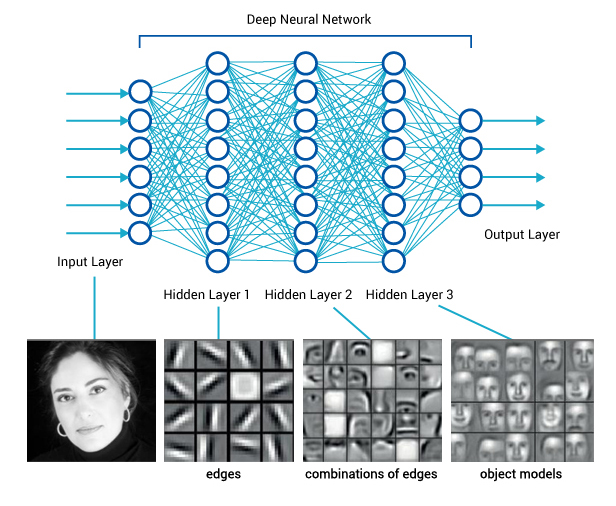
\includegraphics[scale=0.35]{deep_learning_net.jpg}
	  \end{center}
	\end{frame}

  \subsection{D-GEX Architecture}
  \begin{frame}
    \frametitle{D-GEX - 1}
    D-Gex: A mult-task multi-layed feedforward neural network
    \begin{figure}
      \centering
      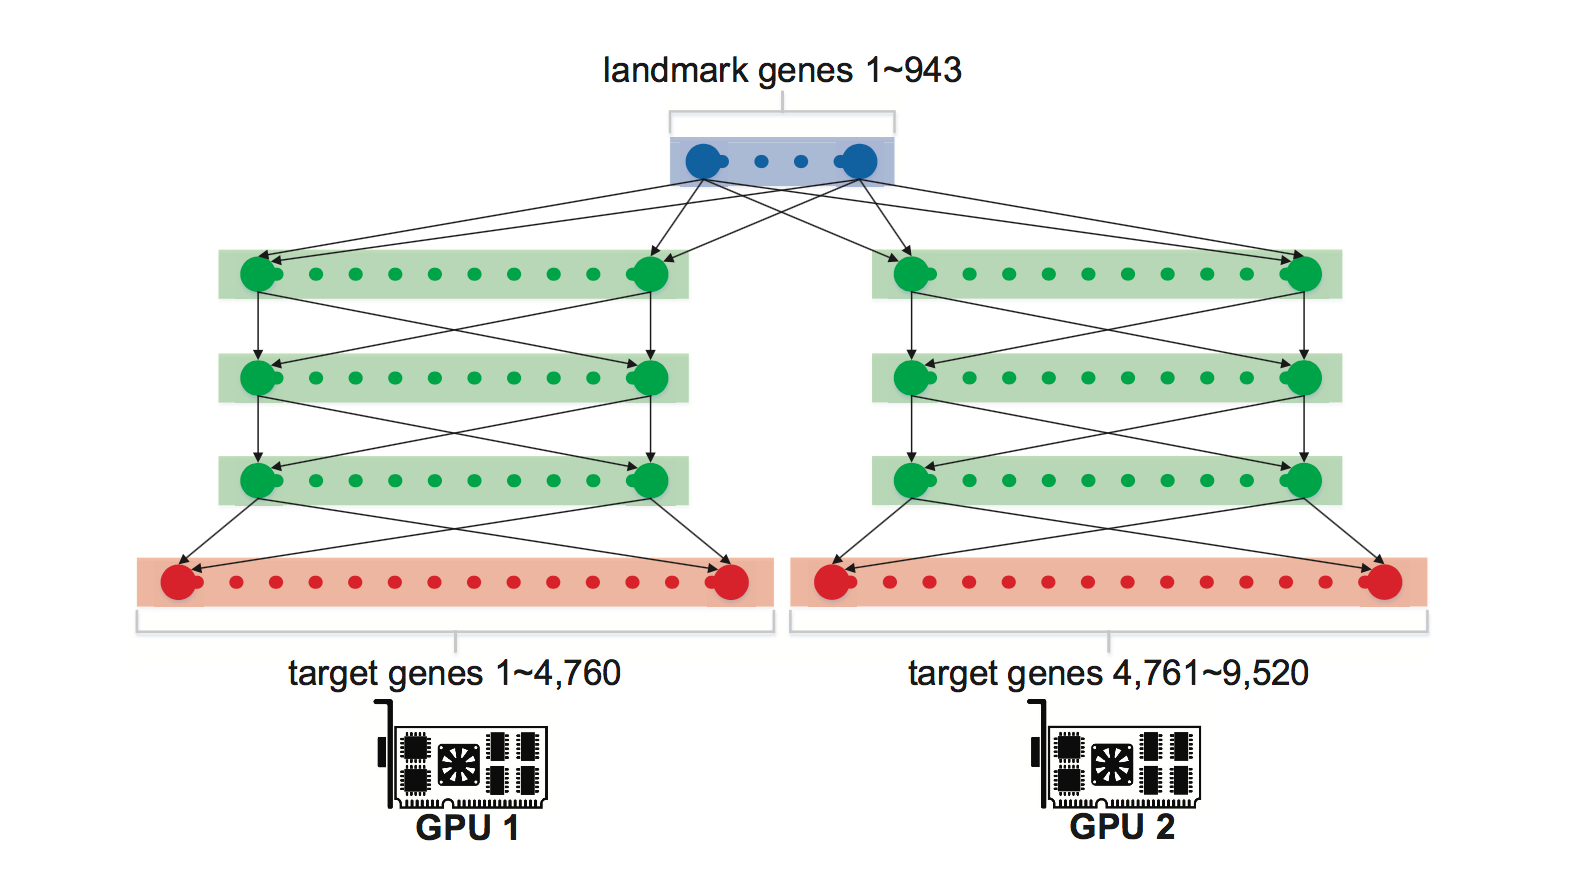
\includegraphics[scale=0.35]{figures/dgexarch.png}
    \end{figure}
    953 hidden units(one for each landmark gene)\newline
    9520 output units, divided in two due to capicity constraints
  \end{frame}

  \subsection{D-GEX Architecture}
  \begin{frame}
    \frametitle{D-GEX - 2}
    The ouput of the hidden unit $j$ in the hidden layer $l$ is given by:
    \begin{equation*}
      o_j^{l} = f(\sum_{i=1}^H \omega_{i,j}^{l-1}o_i^{l-1} + b_j^{l-1})
    \end{equation*}
    $f(x)$ is a non-linear activation function that in our case has been chosen
    as the hyperbolic tangent\newline
    We try the learn ${w_{ij}, b_{j}}$ by minimizing the sum of mean squared errors for each
    output unit($t$)
    \begin{equation*}
      E = \sum_{t=1}^T \left [ \frac{1}{N} \sum_{i=1}^N (y_{i(t)} - \hat{y}_{i(t)})^2 \right ]
    \end{equation*}
  \end{frame}

  \subsection{D-GEX Training}
  \begin{frame}
    \frametitle{D-GEX - Training}
    The training follows the standard back-propagation algorithm, with some
    tricks:
    \begin{itemize}
      \item \textbf{Dropout}: Regularization and model averaging
      \item \textbf{Momentum gradient descent}: Use velocity to update parameters
      \item \textbf{Normalized Initialization:} Initial parameters sampled from a uniform distribution
      \item \textbf{Learning Rate}: $5*10^{-4}$ or $3*10^{-4}$ and decreased according to the training error
      \item \textbf{Model Selection}: 200 epochs and evaluated against the dataset after each epoch
    \end{itemize}
  \end{frame}

  \subsection{Linear Regression}
	\begin{frame}
	  \frametitle{Linear Regression}
    \textbf{Idea}: Train a \textbf{linear} model \textbf{for each} target gene $t$:
    \begin{equation*}
      F_t(x) = w_{t}^T x + b_t
    \end{equation*}
    where $w_{t}^T x$ and $b_t$ are the model parameters associated to $t$:
    \begin{equation}
      (w_t, b_t) = \argmin \limits_{w,b} \frac{1}{N} \sum_{i=1}^N (y_{it} - w_t^T x_i - b_t)^2
    \end{equation}
    For regularization we introduce the L1 and L2 norms:
    \begin{equation}
      (w_t, b_t) = \argmin \limits_{w,b} \frac{1}{N} \sum_{i=1}^N (y_{it} - w_t^T x_i - b_t)^2 + \lambda ||w_t||_1
    \end{equation}
    \begin{equation}
      (w_t, b_t) = \argmin \limits_{w,b} \frac{1}{N} \sum_{i=1}^N (y_{it} - w_t^T x_i - b_t)^2 + \lambda ||w_t||_2
    \end{equation}
    L(1) is currently used in LINCS\newline
    $\lambda$ is tuned on the GEO-va and 1000G-va datasets.
	\end{frame}

  \subsection{KNN}
	\begin{frame}
	  \frametitle{KNN-GE}
    \begin{itemize}
      \item Non-parametric, instance based algorithm
      \item For any testing data, the \textit{k-nearest} neighbors based on a certain
      distance metric(euclidean) are used for the prediction(average)
      \item \textbf{Problem: } Bias due to duplicated samples in the data(DGE)
      \item \textbf{Solution: } Do not query the $k$ nearest sample but the $k$
      nearest genes
      \item \textbf{Pros: } No prior assumption on the model, high capability to
      model non linear pattern
      \item $k$ is tuned on the GEO-va and 1000G-va datasets.
    \end{itemize}
	\end{frame}

  \subsection{Datasets}
	\begin{frame}
	  \frametitle{Datasets - 1}
	  The datasets used are: \newline
    \begin{itemize}
      \item \textbf{GEO Expression Data}
      \begin{itemize}
        \item 129158 gene expression profiles from \textbf{Affymetrix microarray platform}
        \item Normalization: quantile normalization(joint) + duplicate removal
      \end{itemize}

      \item \textbf{GTEx Expression Data}
      \begin{itemize}
        \item 2921 gene expression profiles from \textbf{Illumina RNA-Seq platform}
        \item Normalization: quantile normalization(joint)
      \end{itemize}

      \item \textbf{1000 Genome expression data}
      \begin{itemize}
        \item 462 gene expression profiles from \textbf{Illumina RNA-Seq platform}
        \item Normalization: quantile normalization(joint)
      \end{itemize}
    \end{itemize}
	\end{frame}


  \subsection{Datasets2}
	\begin{frame}
    \frametitle{Datasets - 2}
    For the \textbf{microarray} platform(Affymetrix):
    \begin{itemize}
      \item \textbf{GEO} dataset
      \item 80 \% for training(GEO-tr), 10 \% validation(GEO-va), 10 \% testing(GEO-te)
    \end{itemize}
    \vspace{0.5cm}
    For the \textbf{RNA-Seq} platform:
    \begin{itemize}
      \item The \textbf{GEO-tr} dataset was used for training
      \item The \textbf{1000G}-va dataset was used for validation
      \item The \textbf{GTEx}-te was used for testing
    \end{itemize}
  \end{frame}

  \subsection{RNA-SEQ-1}
  \begin{frame}
    \frametitle{Something on RNA-Seq - 1}
      \begin{itemize}
        \item Developed in \textbf{2008}
        \item Affymetrix Oligonucleotides microarray $\sim$ 2000
        \item cDNA microarray $\sim$ 1995
      \end{itemize}
      \begin{figure}
        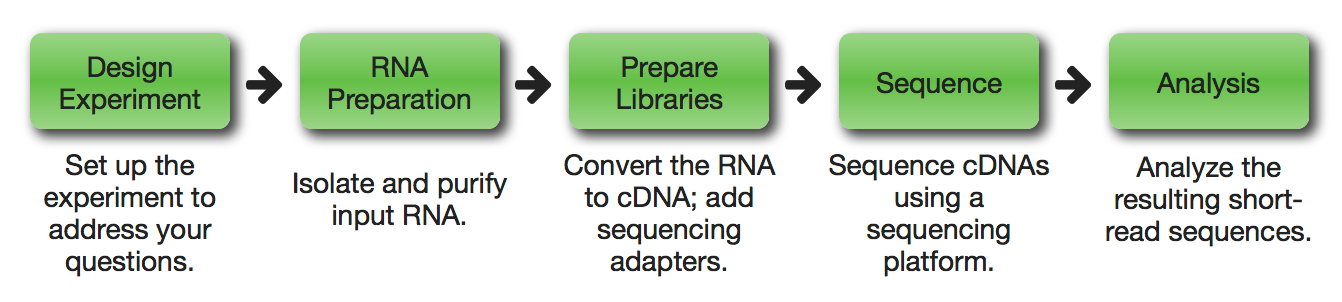
\includegraphics[scale=0.45]{figures/rnaseq.png}
      \end{figure}
  \end{frame}

  \subsection{RNA-SEQ-2}
  \begin{frame}
    \frametitle{Something on RNA-Seq - 2}
      \begin{figure}
        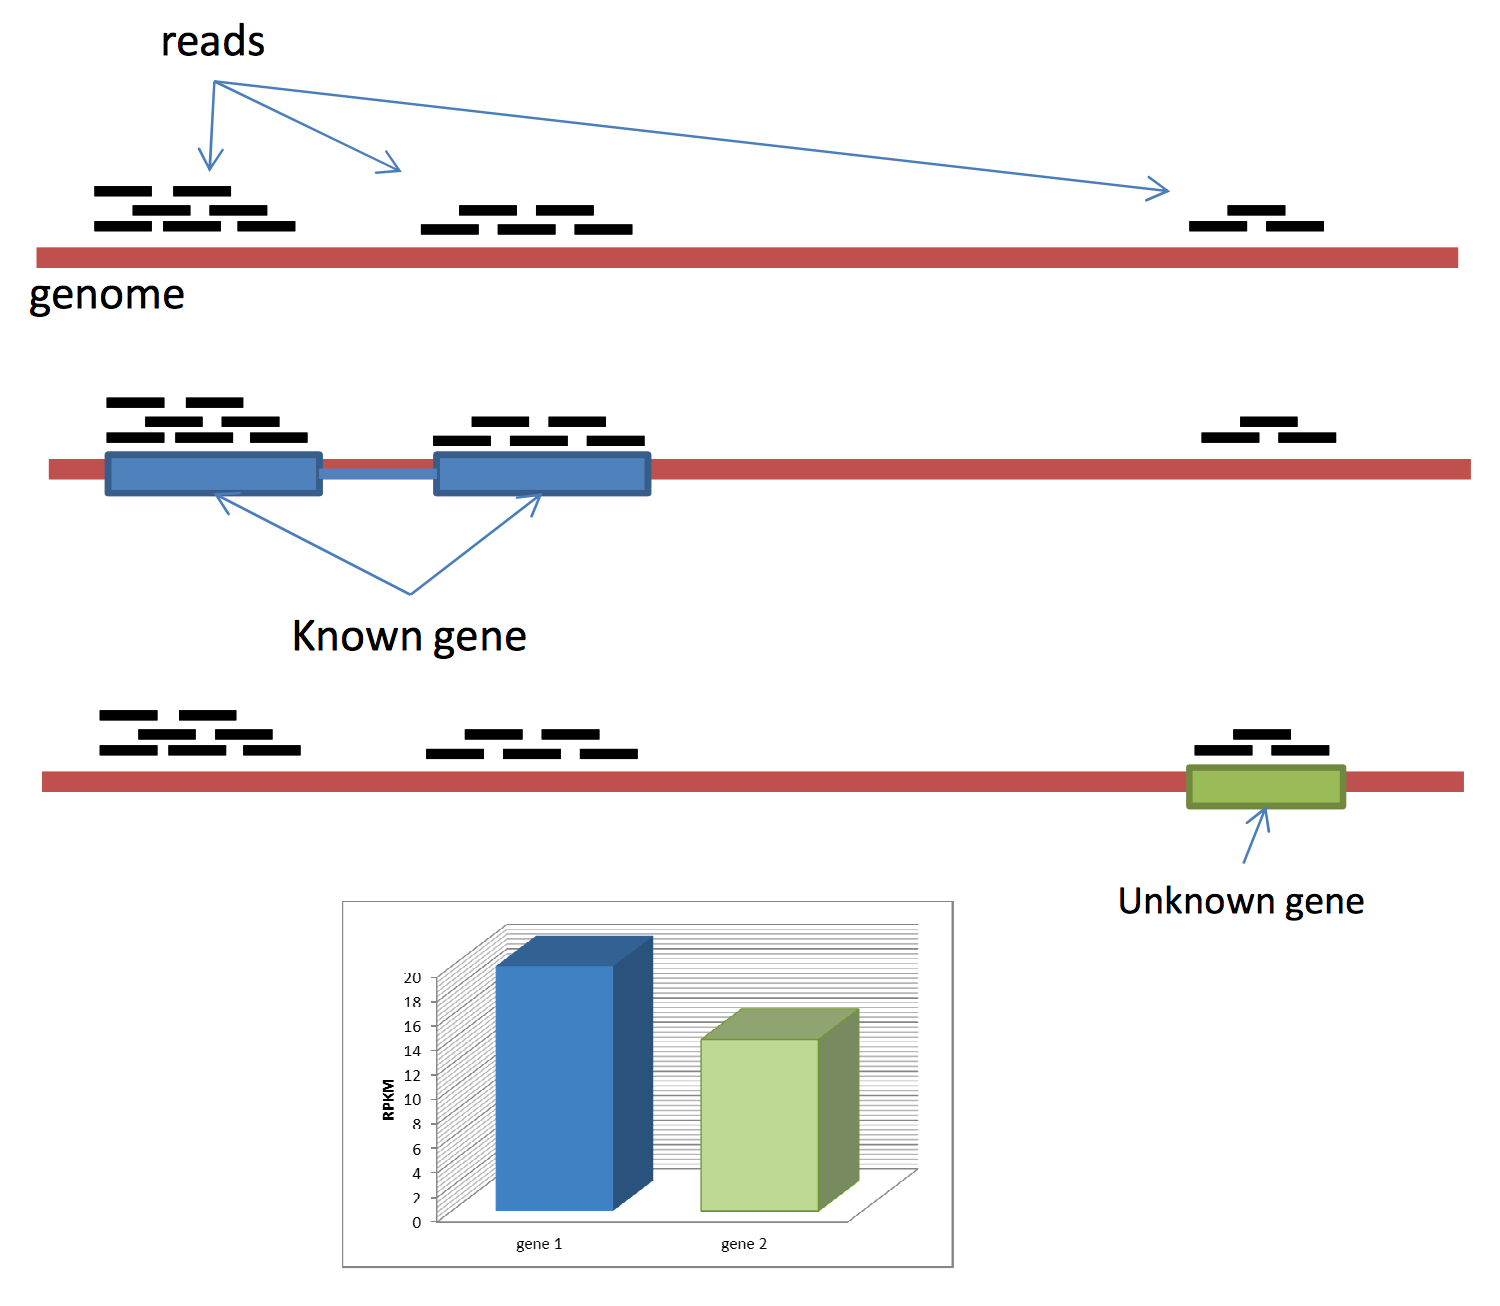
\includegraphics[scale=0.3]{figures/rnaseq2.png}
      \end{figure}
  \end{frame}


  \section{Results and Interpretation}

    \subsection{Performance GEO}
    \begin{frame}
    	\frametitle{Performance on GEO - 1}
    	The best performance of DGEx is achieved with a dropout rate of 10 \%\newline
      \begin{figure}
        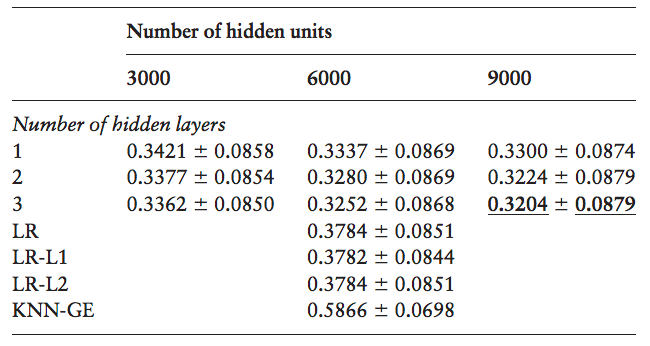
\includegraphics[scale=0.7]{figures/res-geo.png}
      \end{figure}
      Relative improvement: 15.33\% vs LR and 45.38\% vs KNN
    \end{frame}

    \subsection{Performance GEO 2}
    \begin{frame}
      \frametitle{Performance on GEO - 2}
      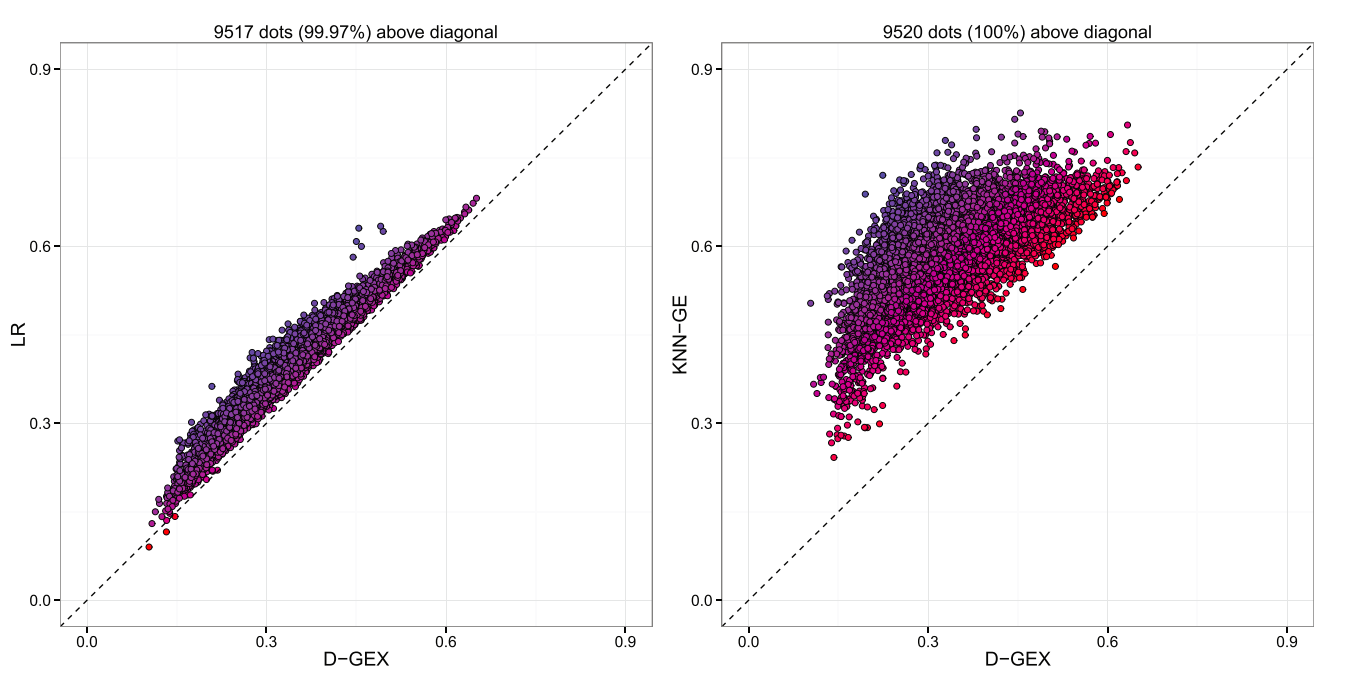
\includegraphics[scale=0.47]{figures/res-geo2.png}
    \end{frame}

    \subsection{Performance GTEX}
    \begin{frame}
      \frametitle{Performance on GTEx}
      Cross-platform scenario: reduced predictive power!
      \begin{figure}
        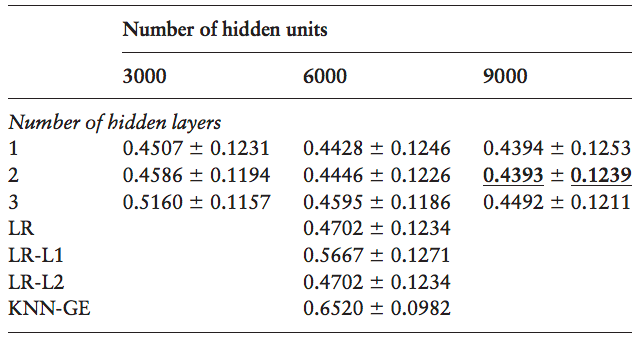
\includegraphics[scale=0.7]{figures/res-gtex.png}
      \end{figure}
      Relative improvement: 6.57\% vs LR and 32.63\% vs KNN
    \end{frame}

    \subsection{Performance GTEx 2}
    \begin{frame}
      \frametitle{Performance on GTEx - 2}
      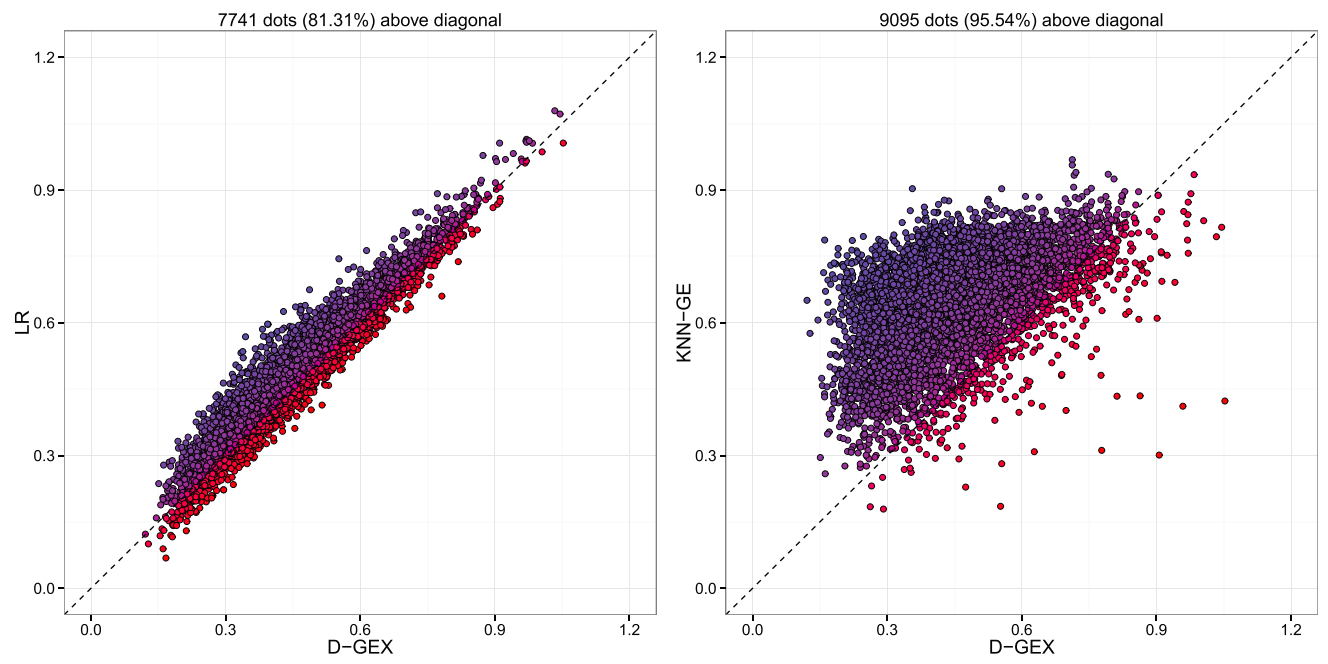
\includegraphics[scale=0.47]{figures/res-gtex2.png}
    \end{frame}


    \subsection{Interpretation}
      \begin{frame}
	       \frametitle{Interpretation}
         Interpreting the linear model produced by \textbf{LR} is \textbf{easy}:
         big coefficients indicate a strong dependency between the target and the
         landmark genes.\newline
         \newline
         On the other hand interpreting the model learned by DGEx is much more
         complex!\newline
         No consolidated method exist, the author proposed:
         \begin{itemize}
           \item Major weight visualization
           \item Analysis of the non-linearity captured by the hidden units
         \end{itemize}
      \end{frame}

    \subsection{Interpretation2}
      \begin{frame}
        \frametitle{Major weights visualization}
          Following the idea of LR, try to visualize the more \textbf{important}
          connection between artificial neurons.\newline
          \begin{center}
            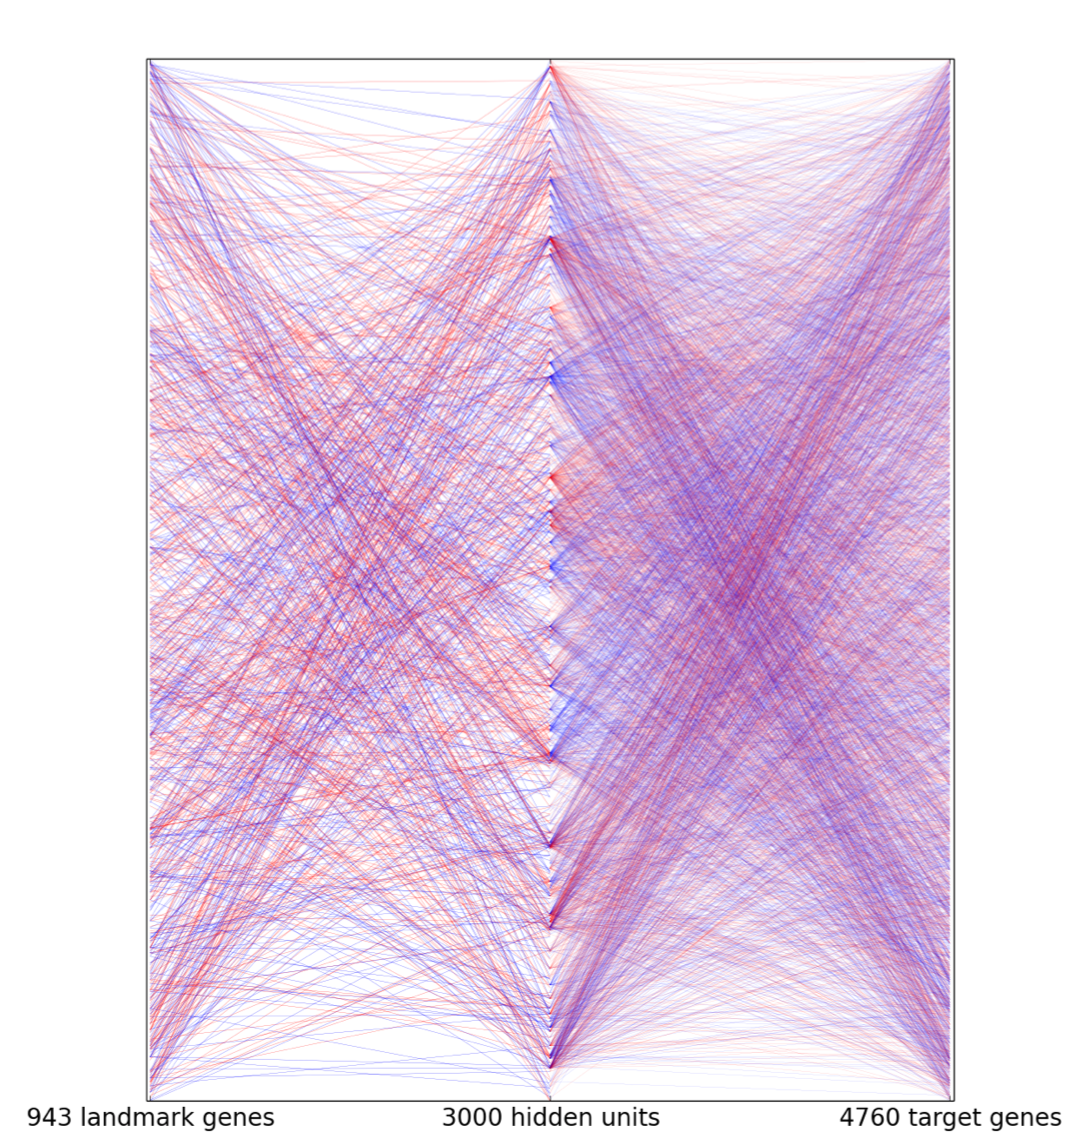
\includegraphics[scale=0.3]{figures/weight1.png}
          \end{center}

      \end{frame}

    \subsection{Interpretation3}
      \begin{frame}
        \frametitle{Non-Linearity Analysis}
          Try to understand if some of the hidden units have captured
          some non-linearity pattern.\newline
          Problem: many neurons in DGEx!\newline
          \newline
          Idea: each hidden unit represent a feature, that is a non-linear
          transformation of the expression of the landmark genes.\newline
          Can a LR model based on this feature achieve better performances than
          a simple LR?\newline
          The author have estimated the (adjusted)$R^2$ between:
          \begin{itemize}
            \item The last hidden layer and the target (features based LR)
            \item The raw input and the target (Simple LR)
          \end{itemize}
          In the first case we achieve a larger $R^2$!
      \end{frame}

    \subsection{Interpretation4}
      \begin{frame}
          \frametitle{Non-Linearity Analysis - Results}
          \begin{figure}
            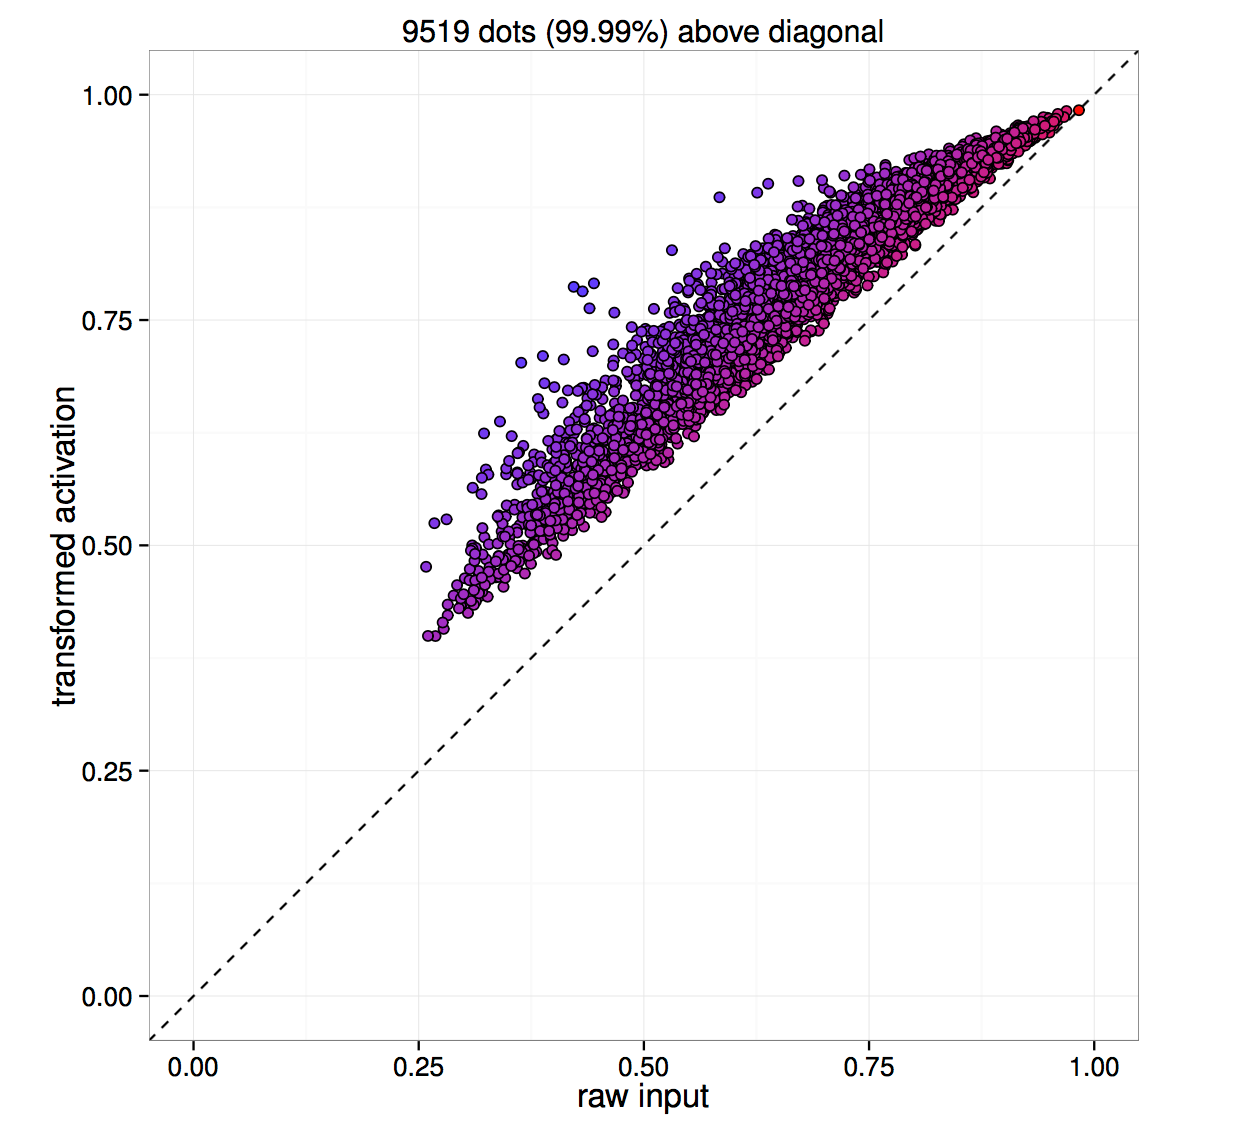
\includegraphics[scale=0.35]{figures/r2.png}
          \end{figure}
      \end{frame}

    \subsection{SW}
        \begin{frame}
          \frametitle{The Software}
            \begin{itemize}
              \item Available at: https://github.com/uci-cbcl/D-GEX
              \item \textbf{Not} user friendly, it a collection of script that model the neural network.
              \item The software permits just to train the network and to evaluate the performance.
              \item Poor documentation: comments in the code???.
              \item Usage of the learned model is up to the final user!
            \end{itemize}

        \end{frame}

    \subsection{Conclusion}
        \begin{frame}
          \frametitle{Conclusions}
          \begin{itemize}
            \item DGEx outperforms LR in a \textbf{single-platform} scenario
            \item DGEx outperforms LR in a \textbf{cross-platform} scenario(dropout)
            \item Interpretation of the learned model lead to the conclusion that
            the network has capture non-linearity pattern in the data(LR probably underfit the data)
            \item Model interpretation in LR is easy while it is very complicated in deep learning settings
          \end{itemize}
          Possible \textbf{improvements}:
          \begin{itemize}
            \item Target genes have been randomly partitioned and each set was
            trained separately using different GPUs
            \item First improvement: perform clustering and the train the model
            \item Target genes sharing similar expression profiles share weights in the NN
            \item Other possibilities: use a larger memory GPU(or multi-GPU techniques)
          \end{itemize}
        \end{frame}

    \subsection{Final}
      \begin{frame}
          \frametitle{}
          \begin{center}
              \begin{figure}
                
\includegraphics[scale=0.5]{figures/thanks.png}
              \end{figure}
          \end{center}
      \end{frame}

\end{document}
